% Messwerte: Alle gemessenen Größen tabellarisch darstellen
% Auswertung: Berechnung geforderter Ergebnisse mit Schritten/Fehlerformeln/Erläuterung/Grafik (Programme)
\section{Auswertung}
\label{sec:auswertung}

\subsection{Fehlerrechnung}
\label{sec:Fehlerrechnung}
Die Fehlerrechnung, für die Bestimmung der Messunsicherheiten, wird mit Uncertainties \cite{uncertainties} gemacht.
Die Formel der Gauß Fehlerfortpflanzung ist gegeben durch
\begin{equation}
    \Delta f=\sqrt{\sum_{i=1}^N\left(\frac{\partial f}{\partial x_i}\right)^2 \cdot\left(\Delta x_i\right)^2}.
    \label{eqn:gauss}
\end{equation}
Für den Mittelwert gilt 
\begin{equation}
    \bar{x} = \frac{1}{N}\sum\limits_{i = 1}^N x_i .
    \label{eqn:mittelwert}
\end{equation}
Der Fehler des Mittelwertes ist gegeben durch 
\begin{equation}
    \Delta \bar{x}=\frac{1}{\sqrt{N}} \sqrt{\frac{1}{N-1} \sum_{i=1}^N\left(x_i-\bar{x}\right)^2}.
    \label{eqn:mittelwertfehler}
\end{equation}

\subsection{Vermessung des Acrylblocks mit einer Schieblehre}
\label{Vermessung des Acrylblocks mit einer Schieblehre}

Der gegeben Acrylblock und dessen Bohrungen wurde wie in \autoref{fig:abmes} dargestellt, vermessen.
Der Block ist $\SI{80.4}{\milli\meter}$ breit , $\SI{150.3}{\milli\meter}$ lang und $\SI{40.3}{\milli\meter}$ tief.
Für die Abstände $a_k$ und $b_k$ und den Durchmesser $d$ der jeweiligen Bohrungen wurde ein Ablesefehler von $\SI{0.05}{\milli\meter}$
angenommen.
\begin{figure}[H]
    \centering
    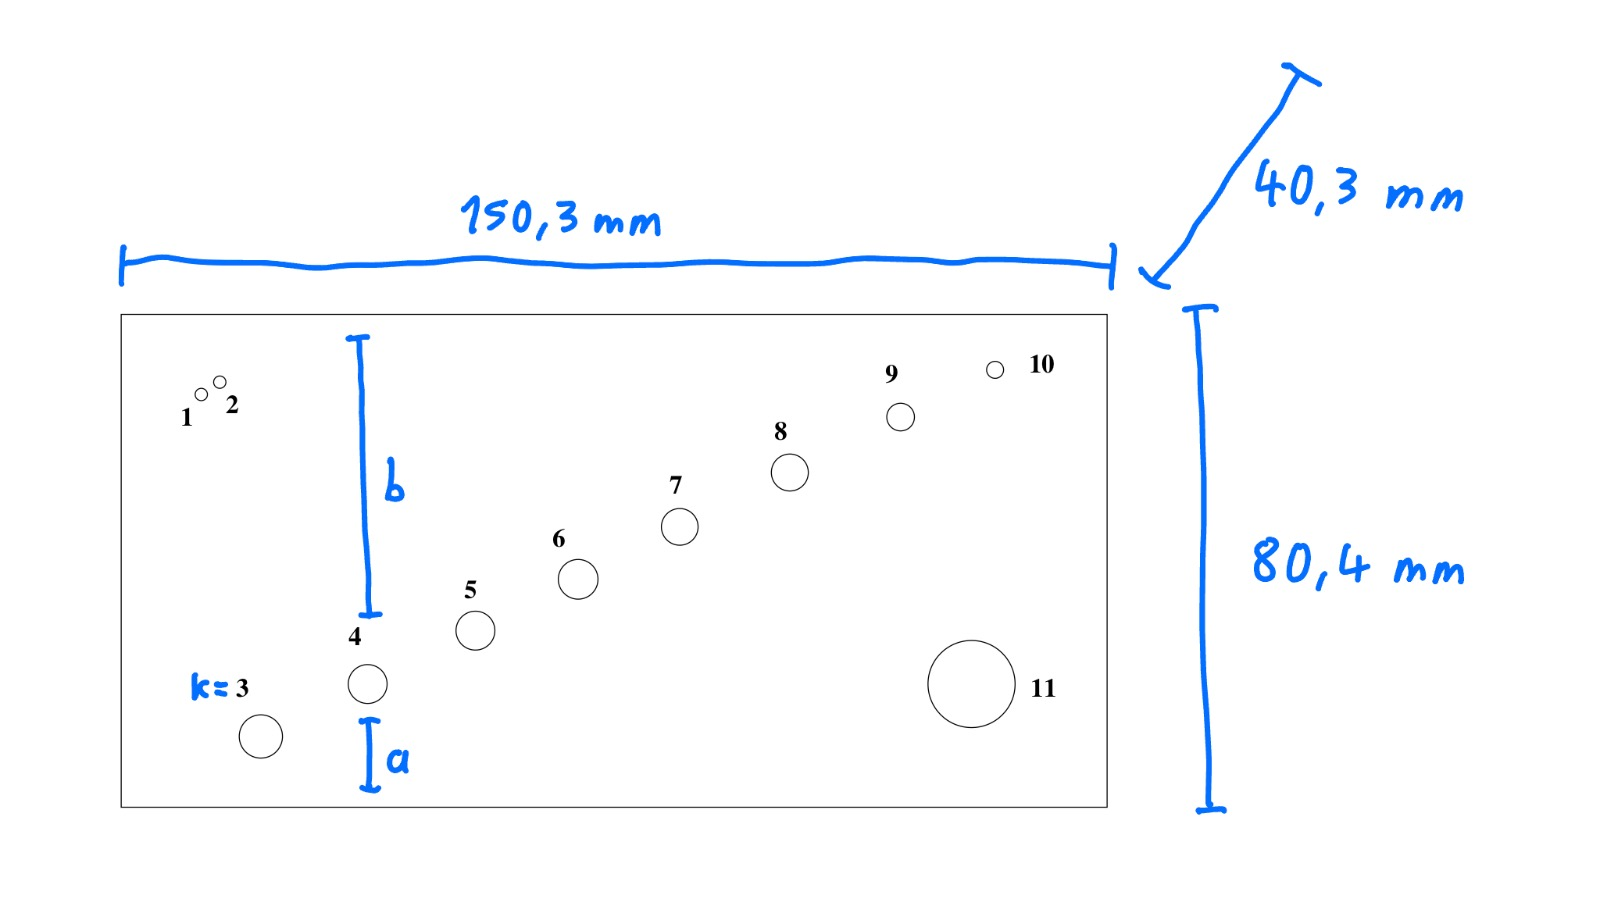
\includegraphics[width=0.9\linewidth]{content/grafik/abmessung.jpg}
	\captionsetup{width=0.765\linewidth}
    \label{fig:abmes}
\end{figure}
Die Messdaten der Abstände $a_k$ und $b_k$ sind in \autoref{tab:lab} zu sehen. 
\begin{table}[H]
    \centering
    \caption{Abmessung der Löcher des Acrylblocks}
    \label{tab:lab}
\begin{tabular}{c c c c}
    \toprule
    Loch & $a_k / \si{\milli\meter}$ & $b_k / \si{\milli\meter}$ & $d / \si{\milli\meter}$\\
    \midrule
    1 &   -  &    -   & 1.45 \\
    2 &   -  &    -   & 1.5 \\
    3 & 13.5 & 61.85 &    6  \\
    4 &21.85 &  54.4 &  4.9  \\
    5 &30.3 &  47.0 &    4  \\
    6 & 38.7 &  39.5 &  2.9  \\
    7 &46.8 &  31.0 &    3  \\
    8 &54.7 &  23.0 &  2.9  \\
    9 & 62.7 & 15.35 & 2.85  \\
    10 & 70.6 &   7.2 & 2.85  \\
    11 &15.2 &  55.8 &  9.5 \\
    \bottomrule
    \end{tabular}
\end{table}

\subsection{Untersuchung der Störstellen des Aceylblocks mit A-Scan}
\label{Untersuchung der Störstellen des Aceylblocks mit A-Scan}
Mit Hilfe des A-Scans wurden die Laufzeiten für die Löcher k = 3 bis k = 9 bestimmt und in der 
\autoref{tab:Laufzeit} aufgetragen. Es wurde dabei von oben gemassen und somit wurden die Laufzeiten für die
$a_k's$ aufgenommen. 
\begin{table}[H]
    \centering
    \caption{Laufzeit von Loch k=3 bis k=9.}
    \label{tab:Laufzeit}
\begin{tabular}{c c}
    \toprule
    Loch & $\text{Laufzeit} t / \si{\micro\second} $\\
    \midrule
     3 & 10.83 \\
     4 &  17.0 \\
     5 &  23.6 \\
     6 &  29.8 \\
     7 &  35.4 \\
     8 &  41.1 \\
     9 &  46.7 \\
    \bottomrule
\end{tabular}
\end{table}
Die Messwerte der Laufzeiten wurden in einem Plot dargestellt, wobei eine lineare Regression der Form 
\begin{equation*}
    a \cdot x + b
\end{equation*}
durchgeführt wurde. Der Plot ist in der \autoref{fig:plot1} dargestellt.

\begin{figure}[H]
	\includegraphics{build/plot1.pdf}
	\captionsetup{width=0.765\linewidth}
	\caption{Die Laufzeit des A-Scans gegen die Abstände $a_k$ aufgetragen und die lineare Ausgleichsgerade.}
	\label{fig:plot1}
\end{figure}

Für die Parameter der Ausgleichsfunktion gilt
\begin{align*}
    a &= \left(2708 \pm 23\right) \si{\meter \per \second}\\
    b &= \left(14 \pm 0.7\right) \si{\milli\meter}.
\end{align*}
Dabei entspricht $a$ der Steigung der Geraden, welche die Schallgeschwindigkeit $\zeta_{\text{exp}}$ in dem Material ist.
Der Literaturwert der Schallgeschwindigkeit $\zeta_{\text{theo}} = \SI{2730}{\meter\per\second}$ wird im weiteren Verlauf für die 
Messungen des A-Scans als auch des B-Scans verwendet.
Der y-Achsen-Abschnitt gibt die Dicke der Anpassungsschicht an. 

Die aufgenommenen Messdaten des A-Scans sind in der \autoref{tab:ascan} dargestellt.
\begin{table}[H]
    \centering
    \caption{Messwerte des A-Scan.}
    \label{tab:ascan}
\begin{tabular}{c c c}
    \toprule
    Loch & $\text{Laufzeit} t / \si{\micro\second} $ & $ d/ \si{mm}$\\
    \midrule
     3 & 14.7 & 63.0 \\
     4 & 23.5 & 55.4 \\
     5 & 32.1 & 47.8 \\
     6 & 40.8 & 40.4 \\
     7 & 48.4 & 32.2 \\
     8 & 56.2 & 24.4 \\
     9 & 64.2 & 16.8 \\
    10 & 73.1 &  8.7 \\
    11 & 17.2 & 56.8 \\
    \bottomrule
\end{tabular}
\end{table}

Um die Abstände, welche mittels Schieblehre bestimmt worden sind, mit den Abständen, welche über einen A-Scan aufgenommen worden sind,
vergleichen zu können, werden die Differenzen der jeweiligen $a_k$ und $b_k$ gemittelt.
Die Messwerte der Schieblehre sind in der \autoref{tab:lab} aufgelistet und die des A-Scans in der \autoref{tab:ascan}.
Für die Mittel der Differenzen ergeben sich die Werte
\begin{align*}
\bar{\increment a_k} &= \SI{1.761}{\milli\meter} \\
\bar{\increment b_k} &= \SI{3.719}{\milli\meter}.
\end{align*}

\subsection{Untersuchung der Störstellen des Aceylblocks mit B-Scan}
\label{sec:Untersuchung der Störstellen des Aceylblocks mit B-Scan}

Mittels des B-Scan wurden Aufnahmen von der oberen und der unteren Kante des Acryl-Blocks durchgeführt.
Diese sind in den \autoref{fig:oben} und \autoref{fig:unten} zu sehen. Anhand des Cursors können die jeweiligen Störstellen 
lokalisiert werden.

\begin{figure}[H]
    \centering
	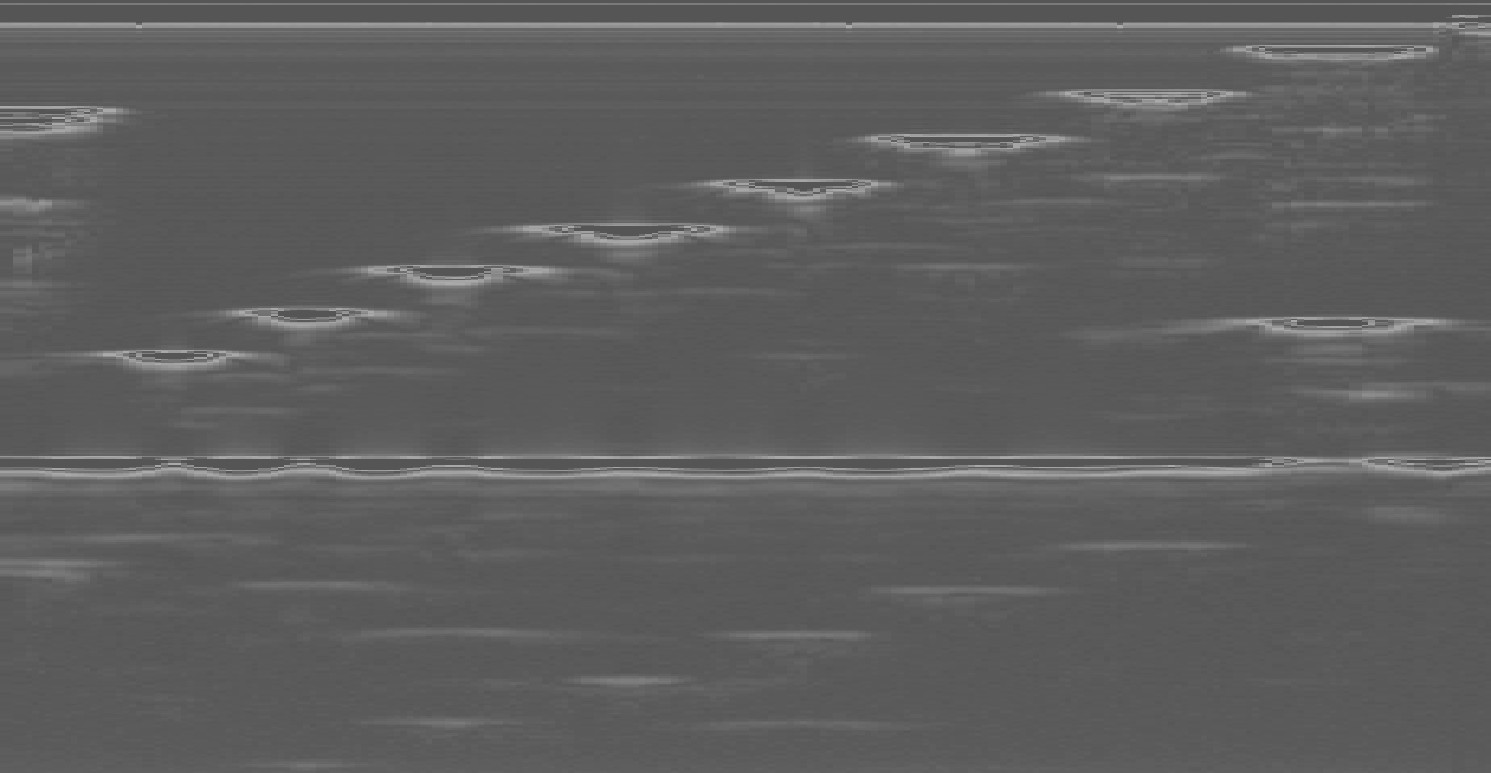
\includegraphics[width=0.8\linewidth]{data/US1_daten/b_scan_oben.jpg}
    \captionsetup{width=0.765\linewidth}
	\caption{Abbildung des Acrylblocks mit B-Scan.}
	\label{fig:oben}
\end{figure}

\begin{figure}[H]
    \centering
	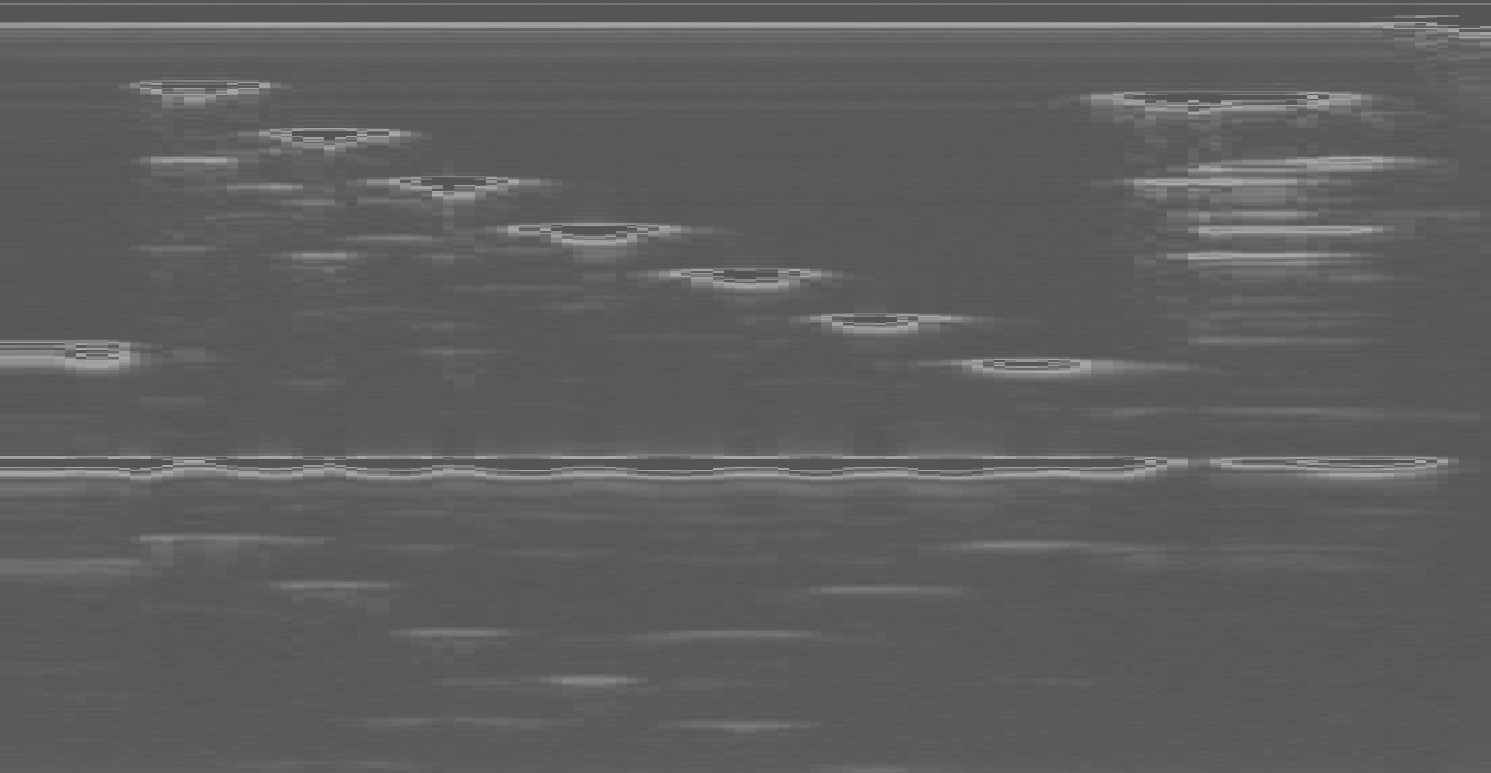
\includegraphics[width=0.8\linewidth]{data/US1_daten/b_scan_u.jpg}
    \captionsetup{width=0.765\linewidth}
	\caption{Abbildung des Acrylblocks mit B-Scan.}
	\label{fig:unten}
\end{figure}

Die Messwerte des B-Scan sind in der \autoref{tab:bscan} aufgetragen. Für $k =10$ konnte kein Wert aufgenommen werden, daher wird dieser
im Folgenden ignoriert.
\begin{table}[H]
    \centering
    \caption{Messwerte des B-Scan.}
    \label{tab:bscan}
\begin{tabular}{c c c}
\toprule
Loch & $\text{Laufzeit} t / \si{\micro\second} $& $ d/ \si{mm}$\\
\midrule
 3 & 15.1 & 63.3 \\
 4 & 23.6 & 55.8 \\
 5 & 32.4 & 48.2 \\
 6 & 40.8 & 40.8 \\
 7 & 48.9 & 33.0 \\
 8 & 56.5 & 24.8 \\
 9 & 64.7 & 16.8 \\
10 & - &  9.0 \\
11 & 17.2 & 57.4 \\
\bottomrule
\end{tabular}
\end{table}

Für die Mittel der Differenzen ergeben sich die Werte
\begin{align*}
\bar{\increment a_k} &= \SI{0.539}{\milli\meter} \\
\bar{\increment b_k} &= \SI{3.719}{\milli\meter}.
\end{align*}

\subsection{Untersuchung des Auslösungsverfahrens} % (fold)
\label{sec:Untersuchung des Auslösungsverfahrens}

Die Löcher $k = 1$ und $k = 2$ wurden mittels A-Scan jeweils mit einer $\SI{1}{\mega\hertz}$ Sonde und mit einer
$\SI{2}{\mega\hertz}$ näher betrachet. Die dabei aufgenommen Messergebnisse sind in den \autoref{fig:plot2} und \autoref{fig:plot3}
zu sehen.

\begin{figure}[H]
	\includegraphics{build/plot2.pdf}
	\captionsetup{width=0.765\linewidth}
	\caption{A-Scan für die Löcher $k = 1$ und $k = 2$ mit einer $\SI{1}{\mega\hertz}$ Sonde.}
	\label{fig:plot2}
\end{figure}
In der \autoref{fig:plot2} ist in der nur ein breiter Peak zu sehen, anhand dessen können die beiden Löcher nicht unterschieden werden.

\begin{figure}[H]
	\includegraphics{build/plot3.pdf}
	\captionsetup{width=0.765\linewidth}
	\caption{A-Scan für die Löcher $k = 1$ und $k = 2$ mit einer $\SI{2}{\mega\hertz}$ Sonde.}
	\label{fig:plot3}
\end{figure}
An der Stelle $t = \SI{20}{\micro\second}$ sind zwei eindeutige Peaks zu erkennen, welche den beiden Löchern $k = 1$ und $k = 2$
zugeordent werden können.
% subsection Untersuchung des Auslösungsverfahrens (end)

\subsection{Untersuchung des Brustmodells mittels B-Scan}
\label{sec:Untersuchung des Brustmodells mittels B-Scan}

Das gegeben Brustmodell wurde mittels B-Scan mehrmals untersucht, dabei waren die Messungen nicht alle gut, daher wurden 
die unbrauchbaren Bilder verworfen.

\begin{figure}[H]
    \centering
	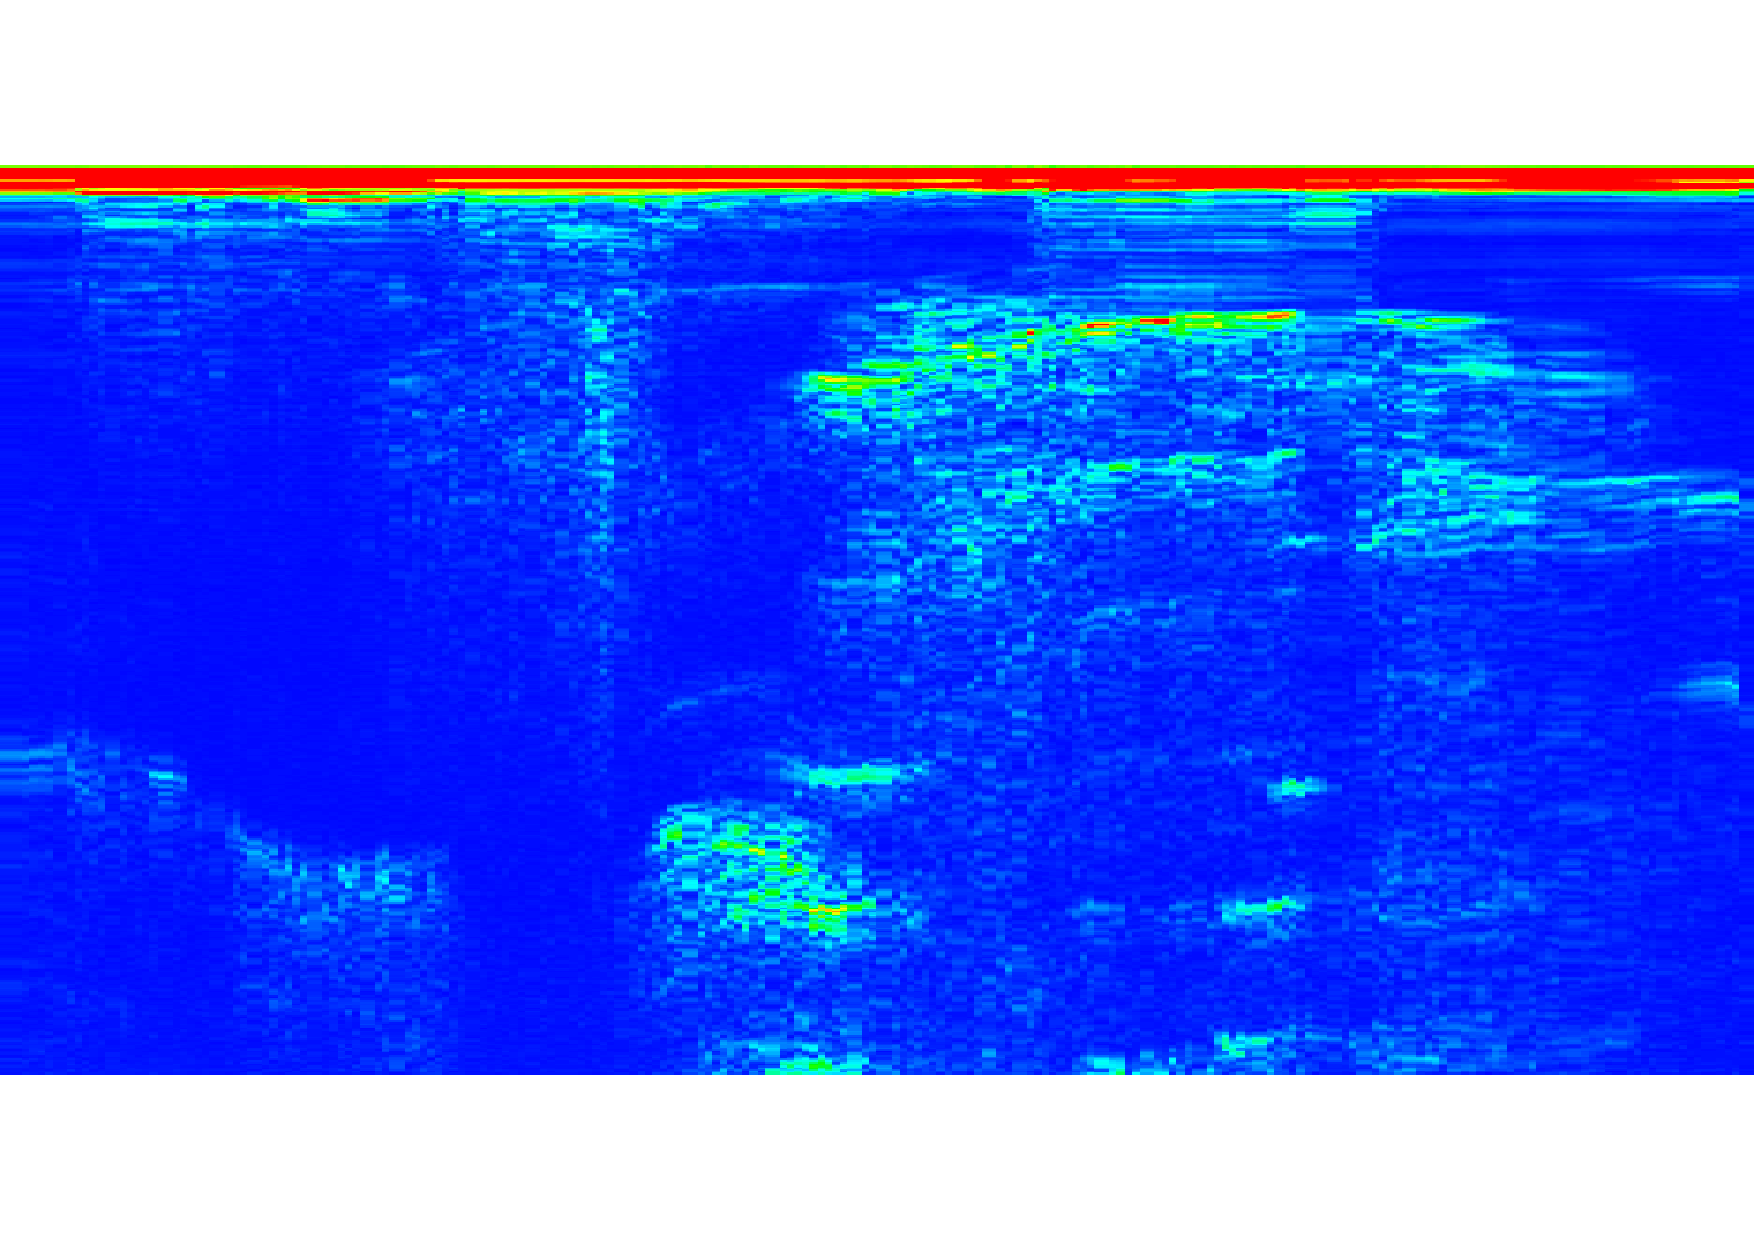
\includegraphics[width=0.8\linewidth]{content/grafik/Tumor_2.pdf}
    \captionsetup{width=0.765\linewidth}
	\caption{Erster B-Scan der Brustmodells.}
	\label{fig:b1}
\end{figure}

\begin{figure}[H]
    \centering
	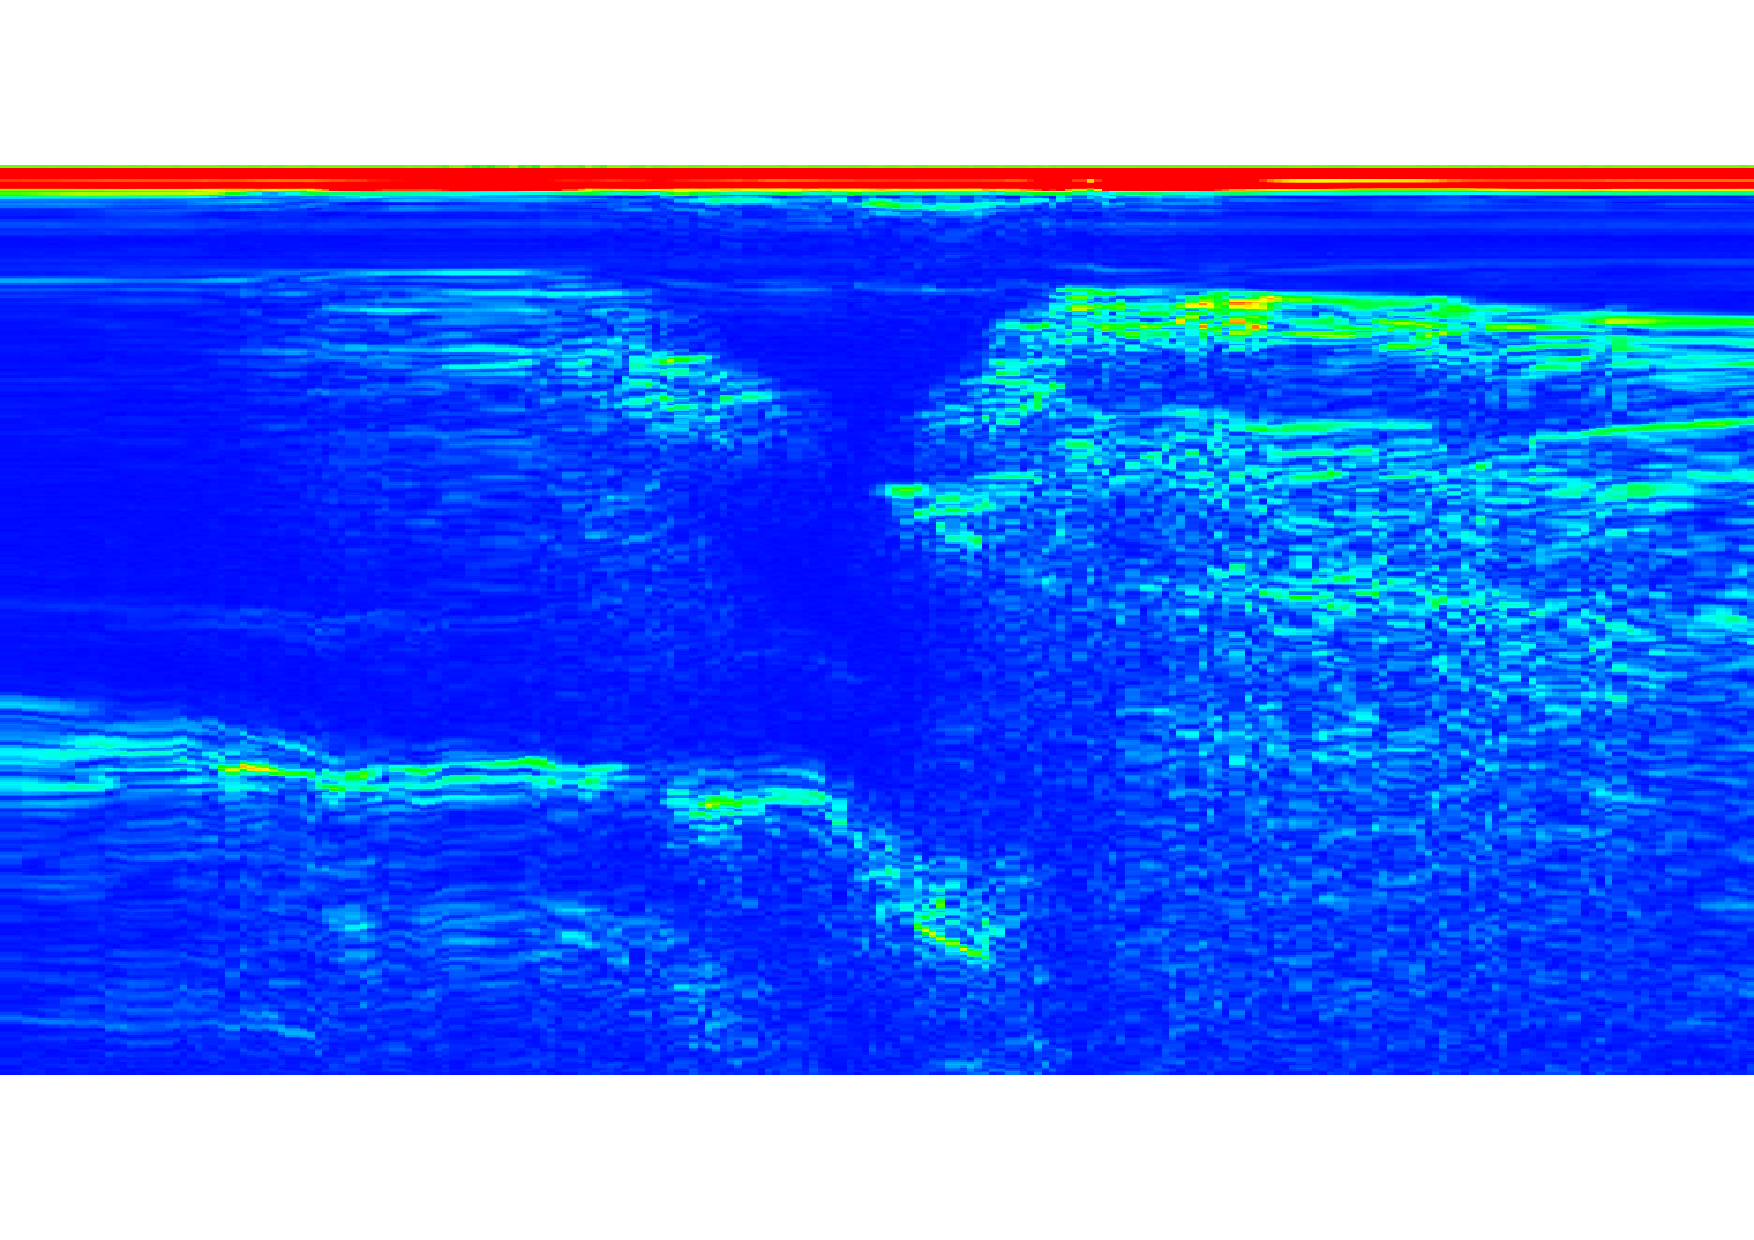
\includegraphics[width=0.8\linewidth]{content/grafik/Super_Tumor.pdf}
    \captionsetup{width=0.765\linewidth}
	\caption{Zweiter B-Scan der Brustmodells.}
	\label{fig:b2}
\end{figure}

Anhand der \autoref{fig:b2} kann gesagt werden, dass es sich bei den zwei oberen Arsenalen, um die gesuchten
Störstellen handelt. Der rechte obere Fleck ist der Tumor, aufgrund der farblichen Erkennung . Der linke Bereich deutet auf eine 
Zyste hin, da diese kein Knoten ist, sondern ein Hohlraum.